\PassOptionsToPackage{hyphens}{url}
\PassOptionsToPackage{colorlinks,linkcolor=darkblue,citecolor=darkblue,urlcolor=darkblue}{hyperref}
\usepackage[utf8]{inputenc}
% T1 gives every font a real underscore glyph at slot 95. OT1 does not: there, the text
% fonts hold a dot accent in that slot (cmss: 2.78pt wide, 6.79pt high, no depth -- it
% sits above the baseline), which is why LaTeX drew \_ as a rule instead. Only the OT1
% typewriter font has a real underscore. With T1 the glyph exists in roman, sans, bold and
% typewriter alike, so \_ looks right everywhere, including the bold table names in the
% schema diagram. lmodern supplies T1-encoded Type 1 fonts (Latin Modern, metrically the
% same as Computer Modern); without it T1 falls back to bitmapped EC fonts.
\usepackage[T1]{fontenc}
\usepackage{lmodern}
\usepackage[english]{babel}
\usepackage[hyphens]{url}
\usepackage{doi}
\usepackage{hyperref}
\usepackage{amsmath}
\usepackage{amssymb}
\usepackage{amsthm}
\usepackage{tikz}
\usepackage{tikzpeople} % \node[alice] {}; and suchlike
\usepackage{natbib}
\usepackage{fancyhdr} % license footer on first page
\usepackage{textcomp} % \textdegree
\usepackage{algorithm}
\usepackage{algpseudocode} % for pseudocode
\usepackage{mdframed}

% The minted package does source code syntax highlighting using Pygments: https://pygments.org/
% Pygments must be installed on your system, e.g. using `pip3.8 install Pygments`.
% pdflatex must be run with option -shell-escape so that it can run pygmentize.
% The minted cache directory is not in git: minted only reads it when passed
% frozencache=true, which we do not, so committing it would achieve nothing while adding a
% new hash-named file on every edit to a listing. To build without Pygments, pass
% finalizecache=true once to write the cache, then frozencache=true to read it, and commit
% the cache that run produced -- from the same minted version that will read it, since
% minted 2.x and 3.x use different cache layouts. -shell-escape is then not needed either.
\usepackage{minted}

% \code{...} is \texttt for identifiers and code fragments, taking its argument literally:
% write \code{has_genre} rather than \texttt{has\_genre}. Unlike \verb it works inside a
% beamer frame -- \verb there needs \begin{frame}[fragile], because beamer re-reads frame
% bodies to build overlays -- and inside the argument of another command. Braces must still
% balance, and it cannot contain other commands, since the argument is detokenised.
\newcommand{\code}[1]{\texttt{\detokenize{#1}}}

\usetikzlibrary{arrows.meta}
\usetikzlibrary{shapes.multipart}
\usetikzlibrary{shapes.callouts}
\usetikzlibrary{decorations.pathreplacing} % {brace} decoration
\usetikzlibrary{fit} % fit= a node around marked cells, to circle them
\usetikzlibrary{shapes.geometric} % the ellipse shape, for circling a value
\tikzstyle{bigarrow}=[very thick,-{Classical TikZ Rightarrow[length=2mm]}]
\tikzstyle{revbigarrow}=[very thick,{Classical TikZ Rightarrow[length=2mm]}-]
\tikzstyle{doublebigarrow}=[very thick,{Classical TikZ Rightarrow[length=2mm]}-{Classical TikZ Rightarrow[length=2mm]}]
\tikzstyle{messageloss}=[very thick,-{Rays[length=8mm,red,line width=4pt]}]
\tikzstyle{crash}=[-{Rays[length=8mm,red,line width=4pt]}]
\tikzstyle{leftloop}=[loop left,out=135,in=225,looseness=10]
\tikzstyle{rightloop}=[loop right,out=45,in=325,looseness=10]
\tikzstyle{op}=[rectangle,fill=white,draw,rotate=270,align=left,font=\footnotesize,minimum height=0.6cm]

% Records the position of the point where it is used, so that a later
% tikzpicture with [remember picture,overlay] can draw relative to it -- used to put
% braces beside particular rows of a table. Needs two LaTeX runs, since the position
% travels via the .aux file. A row's baseline is at the mark; with \arraystretch=1.3
% the row extends 10.92pt above it and 4.68pt below (1.3 x 0.7 and 1.3 x 0.3 of the
% 12pt \footnotesize \baselineskip).
\newcommand{\tikzmark}[1]{\tikz[remember picture,overlay]\coordinate (#1);}

% Like \tikzmark, but keeps the extent of the text rather than recording only a point, so
% that a later [remember picture,overlay] tikzpicture can fit= a shape around it -- a circle
% round a value, or a brace under a whole column. examples/render.py emits these from its
% `mark:` directive, naming the header cell <prefix>0 and the data rows <prefix>1 upwards.
% A small cylinder, the conventional picture of a disk or a stored dataset.
\newcommand{\storageSymbol}{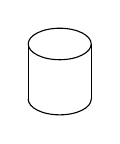
\begin{tikzpicture}%
    \draw (0.4, 0.7) ellipse (0.4 and 0.2);
    \draw (0.0, 0.0) arc (180:360:0.4 and 0.2);
    \draw (0.0, 0) -- (0.0, 0.7);
    \draw (0.8, 0) -- (0.8, 0.7);
\end{tikzpicture}}

\newcommand{\tikzmarknode}[2]{%
    \tikz[remember picture,baseline=(#1.base),inner sep=0pt,outer sep=0pt]%
        \node[anchor=base] (#1) {#2};}

\urlstyle{sf}
\newcounter{inlineslides}

\newcommand{\inlineslide}[2]{
    \refstepcounter{inlineslides}
    \pagebreak[3]\vspace{1em}\noindent
    \fbox{
      \begin{minipage}{9cm}
        \begin{center}
          \includeslide[width=9cm,page=0]{#1} \\
        \end{center}
      \end{minipage}
    }
    \hfill
    \begin{minipage}{6cm}
        \vbox to 5.5cm {\raggedright{#2}\vfil}%
        \vspace{1cm}%
        \textsf{Slide \theinlineslides}%
    \end{minipage}
    \par\vspace{1em}\pagebreak[3]
}
\def\inlineslidesautorefname{Slide}%

\definecolor{darkblue}{rgb}{0,0,0.7}
\definecolor{darkgreen}{rgb}{0,0.7,0.0}
\definecolor{lightgrey}{rgb}{0.95,0.95,0.95}

% Exercises and solution notes. See also databases-notes.tex
\newtheorem{exercise}{Exercise}
\def\exerciseautorefname{Exercise}%
\newcommand\supervision[2]{\begin{exercise}#1\end{exercise}}
